\documentclass[10pt,compress,t,notes=noshow, xcolor=table]{beamer}

\input{../../style/preamble}
\input{../../latex-math/basic-math}
\input{../../latex-math/basic-ml}
\input{../../latex-math/ml-interpretable}
% Defines macros and environments

\newcommand{\gh}{\hat{g}}

\title{Interpretable Machine Learning}
% \author{LMU}
%\institute{\href{https://compstat-lmu.github.io/lecture_iml/}{compstat-lmu.github.io/lecture\_iml}}

\begin{document}

% Set style/preamble.Rnw as parent.

% Load all R packages and set up knitr

% This file loads R packages, configures knitr options and sets preamble.Rnw as
% parent file
% IF YOU MODIFY THIS, PLZ ALSO MODIFY setup.Rmd ACCORDINGLY...

% Defines macros and environments

\titlemeta{
Local Explanations: Lime
}{
Examples
}{
figure/lime_credit_ice2.pdf
}{
\item See real-world data examples
\item See application to image and text data
}

% Prerequisite: le-intro

% ------------------------------------------------------------------------------
\begin{framev}[align=top]{Example: Credit Scoring (Tabular Data)}
\begin{itemizeM}
\item \textbf{Black-box model $\fh_{bad}$:} SVM with RBF kernel (predicts probability of bad credit risk)
\item \textbf{Instance to explain $\xv$:} First row in the dataset, with $\fh_{bad}(\xv) = 0.658$
\begin{scriptsize}
\begin{tabular}{r l r l r r r l l l}
\hline
duration & sex & credit.amount & purpose & housing & age & saving & checking & ... \\
\hline
48 & female & 5951 & radio/TV & own & 22 & little & moderate & ... \\
\hline
\end{tabular}
\end{scriptsize}
\item \textbf{Surrogate model:} LASSO, restricted to 5 non-0 feats (via regularization)
\item \textbf{Training data for surrogate:} Samples $\zv$, weighted by Gower dist. to $\xv$
\end{itemizeM}
\pause
\splitVTT{
\spacer[0.6]
\begin{itemizeM}
\item \textbf{Prediction:} \\
$\gh(\xv) = 0.640$ vs. $\fh_{bad}(\xv) = 0.658$
\item[$\leadsto$] $\gh$ provides good local approx. of $\fh_{bad}$, but omits several features
\item[$\leadsto$] Small mismatch reflects trade-off: \\
\textbf{interpretability vs. fidelity}
\end{itemizeM}
}{
\spacer[0]
\image{figure/lime_credit.pdf}
\spacer[0]
}
\textbf{Interpretation:} Prediction is mainly driven by loan duration, with small positive effect from sex and credit.amount, and negative contributions from housing and purpose.
\end{framev}


\begin{framev}[align=top]{Example on Credit Dataset (cont'd)}
\begin{itemizeM}
\item 2D ICE plots (pred. surface plots) for \texttt{duration} and \texttt{credit.amount}
\item Illustration how $\gh$ linearly approximates nonlinear decision surface of $\fh_{bad}$
\end{itemizeM}
\splitVTT{
\spacer[0]
\image{figure/lime_credit_ice1.pdf}
\spacer[0]
}{
\spacer[0]
\image{figure/lime_credit_ice2.pdf}
\spacer[0]
}
\begin{itemizeM}
\item \textbf{Left:} 2D ICE plot of $\fh_{bad}$ showing decision surface
\item \textbf{Right:} Linear approximation by surrogate model $\gh$. \\
$\leadsto$ White dot indicates input $\xv$ to be explained \\
$\leadsto$ Histograms show marginal distribution of features in training data % training data \( \Xmat \).
\end{itemizeM}
\end{framev}

%\begin{frame}[containsverbatim,allowframebreaks]{Bike Sharing Dataset}
%\vspace{-.3cm}
%
%\begin{center}
%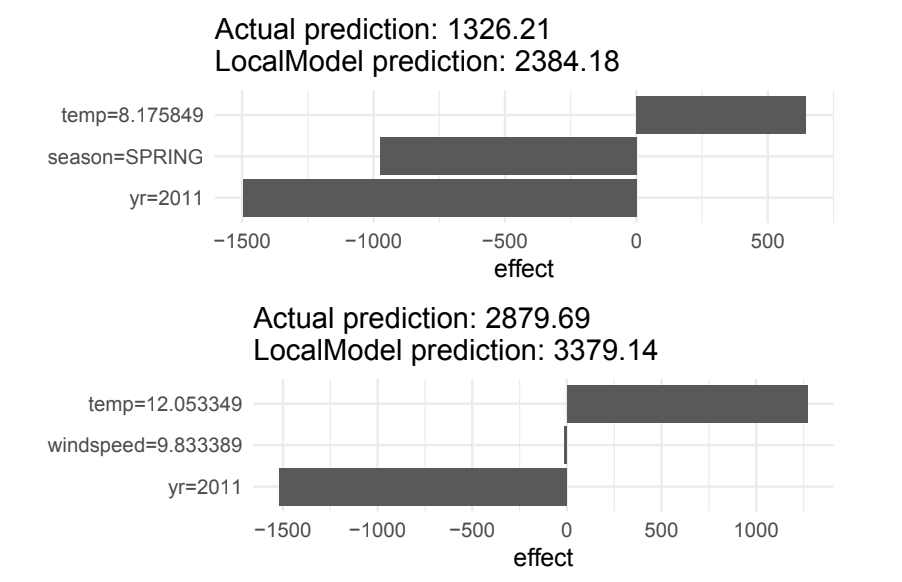
\includegraphics[width=0.7\textwidth]{figure/bike-figure.png}
%\end{center}
%
%\footnotesize \textbf{Figure:} LIME for two example instances of the bike sharing dataset.
%
%\normalsize
%\vspace{0.2cm}
%The plots show the feature effect of the sparse linear model, i.e. the model coefficients times the feature value of the instance.
%Warmer temperature has a positive effect on the prediction,
%while the year 2011 has a large negative effect as well as the springtime.
%\end{frame}

\begin{framev}[align=top]{LIME for Text Data \furtherreading{IAN2019}}
LIME can also be applied to text data:
\begin{itemizeM}
\item Raw text representations:
\begin{itemizeS}
\item Binary vector indicating the presence or absence of a word
\item A vector of word counts
\end{itemizeS}
\item Examples for \textit{``This text is the first text."} and \textit{``Finally, this is the last one."}:
\begin{center}
\begin{tabular}{c|c|c|c|c|c|c|c}
this & text & is & the & first & finally & last & one \\
\hline
1 & 2 & 1 & 1 & 1 & 0 & 0 & 0 \\
1 & 0 & 1 & 1 & 0 & 1 & 1 & 1 \\
\end{tabular}
\end{center}
\item \textbf{Sampling}: Randomly set the entry of individual words to $0$; equal to removing all occurrences of this word in the text.
\item \textbf{Proximity}: Exponential kernel with cosine distance.
\begin{itemizeS}
\item Neglects words that do not occur in both texts
\item Measures the distance irrespective of the text size
\end{itemizeS}
\end{itemizeM}
\end{framev}


\begin{framev}[align=top]{LIME for Text Data (cont'd) \furtherreading{IAN2019}}
\begin{itemizeM}
\item Random forest classifier labeling movie reviews from IMDB
\begin{itemizeS}
\item \textcolor{blue}{0}: negative
\item \textcolor{orange}{1}: positive
\end{itemizeS}
\item Surrogate model is a sparse linear model
\end{itemizeM}
\imageC[0.9]{figure/lime_movier}
\spacer[0.25]
Words like ``worst`` or ``waste`` indicate negative review while words like ``best`` or ``great`` indicate positive review
\end{framev}


\begin{framev}[align=top]{LIME for image data}
\splitVTT[0.7]{
LIME also works for image data:
\begin{itemizeM}
\item \textbf{Idea}: Each obs. is represented by a binary vector indicating the presence or absence of superpixels \furtherreading{ACHANTA2012}
\item Superpixels are interconnected pixels with similar colors (absence of a single pixel might not have a (strong) effect on the prediction)
\item \textbf{Warning}: Size of superpixels needs to be determined before the segmentation takes place
\item \textbf{Sampling}: Randomly switching some of the super pixels ``off", i.e., by coloring some superpixels uniformly
\end{itemizeM}
}{
\spacer[0]
\begin{center}
\image{figure/superpixel_woman}
Example for superpixels of different sizes
\end{center}
}
\end{framev}


\begin{framev}[align=top]{LIME for image data (cont'd) \furtherreading{RIBEIRO2016}}
\begin{itemizeM}
\item Explaining prediction of pre-trained inception neural network classifier
\item \textbf{Sampling}: Graying out all superpixels besides 10 superpixels
\item \textbf{Surrogate}: Locally weighted sparse linear models
\item \textbf{Proximity}: Exponential kernel with euclidean distance
\end{itemizeM}
% https://lime-ml.readthedocs.io/en/latest/lime.html#module-lime.lime_image
\begin{center}
\image[0.8]{figure/lime-images}\\
Top 3 classes predicted
\end{center}
\end{framev}
\endlecture
\end{document}
